Цилиндр вписан в правильную четырёхугольную призму. Радиус основания и высота цилиндра равны 3. Найдите площадь боковой поверхности призмы.
Ответ: ____.
\documentclass[tikz,border=5pt]{standalone}

\begin{document}

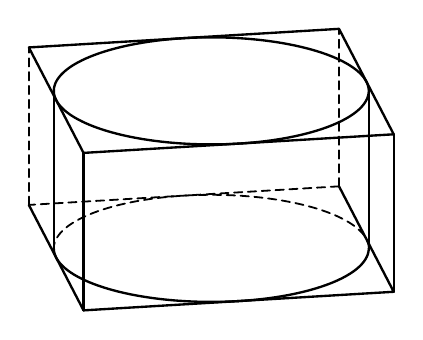
\begin{tikzpicture}[
    x={(1cm,0cm)},
    y={(0cm,0.34cm)},
    z={(0cm,1cm)},
    line cap=round,
    line join=round,
    visible/.style={line width=0.85pt},
    hidden/.style={
        line width=0.65pt,
        dashed,
        dash pattern=on 3pt off 2pt
    }
]

% =========================================================
% Параметры рисунка
% =========================================================

\def\r{2}       % радиус основания цилиндра
\def\H{2}       % высота цилиндра и призмы
\def\phi{10}    % угол поворота квадратного основания

% Радиус описанной окружности квадрата
\pgfmathsetmacro{\R}{sqrt(2)*\r}

% =========================================================
% Вершины нижнего основания призмы
% =========================================================

\coordinate (A0) at
    ({\R*cos(45+\phi)},{\R*sin(45+\phi)},0);

\coordinate (A1) at
    ({\R*cos(135+\phi)},{\R*sin(135+\phi)},0);

\coordinate (A2) at
    ({\R*cos(225+\phi)},{\R*sin(225+\phi)},0);

\coordinate (A3) at
    ({\R*cos(315+\phi)},{\R*sin(315+\phi)},0);

% =========================================================
% Вершины верхнего основания призмы
% =========================================================

\coordinate (B0) at
    ({\R*cos(45+\phi)},{\R*sin(45+\phi)},\H);

\coordinate (B1) at
    ({\R*cos(135+\phi)},{\R*sin(135+\phi)},\H);

\coordinate (B2) at
    ({\R*cos(225+\phi)},{\R*sin(225+\phi)},\H);

\coordinate (B3) at
    ({\R*cos(315+\phi)},{\R*sin(315+\phi)},\H);

% =========================================================
% Невидимое заднее ребро нижнего основания
% =========================================================

\draw[hidden] (A0)--(A1);

% =========================================================
% Невидимые вертикальные рёбра
% =========================================================

\draw[hidden] (A0)--(B0);
\draw[hidden] (A1)--(B1);

% =========================================================
% Невидимая часть нижней окружности цилиндра
% =========================================================

\draw[hidden]
    plot[
        domain=0:180,
        samples=100,
        variable=\t
    ]
    ({\r*cos(\t)},{\r*sin(\t)},0);



% =========================================================
% Видимые рёбра нижнего основания
% =========================================================

\draw[visible] (A1)--(A2)--(A3)--(A0);

% =========================================================
% Видимые вертикальные рёбра призмы
% =========================================================

\draw[visible] (A2)--(B2);
\draw[visible] (A3)--(B3);

% =========================================================
% Образующие цилиндра
% =========================================================

\draw[visible] (-\r,0,0)--(-\r,0,\H);
\draw[visible] ( \r,0,0)--( \r,0,\H);

% =========================================================
% Видимая часть нижней окружности цилиндра
% =========================================================

\draw[visible]
    plot[
        domain=180:360,
        samples=100,
        variable=\t
    ]
    ({\r*cos(\t)},{\r*sin(\t)},0);

% =========================================================
% Верхнее основание призмы
% =========================================================

\draw[visible]
    (B0)--(B1)--(B2)--(B3)--cycle;

% =========================================================
% Верхнее основание цилиндра
% =========================================================

\draw[visible]
    plot[
        domain=0:360,
        samples=160,
        variable=\t
    ]
    ({\r*cos(\t)},{\r*sin(\t)},\H);

\end{tikzpicture}

\end{document}

Цилиндр вписан в правильную шестиугольную призму. Радиус основания цилиндра равен \sqrt{3}, а высота призмы равна 2. Найдите площадь боковой поверхности призмы.
\documentclass[tikz,border=5pt]{standalone}

\begin{document}

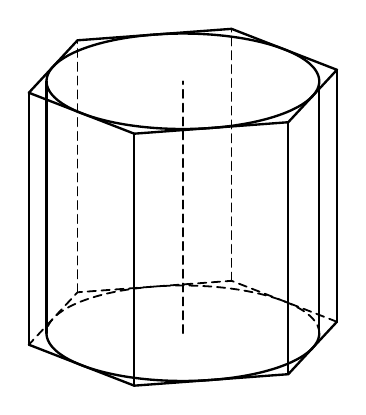
\begin{tikzpicture}[
    x={(1cm,0cm)},
    y={(0cm,0.35cm)},
    z={(0cm,1cm)},
    line cap=round,
    line join=round,
    visible/.style={line width=0.85pt},
    hidden/.style={line width=0.65pt,dashed,dash pattern=on 3pt off 2pt}
]

% =========================================================
% Параметры
% =========================================================

\def\a{2}      % сторона правильного шестиугольника
\def\H{3.2}    % высота призмы
\def\phi{12}   % угол поворота основания

% Радиус вписанной окружности правильного шестиугольника
\pgfmathsetmacro{\r}{sqrt(3)*\a/2}

% =========================================================
% Вершины нижнего основания
% =========================================================

\coordinate (A0) at ({\a*cos(\phi)},      {\a*sin(\phi)},      0);
\coordinate (A1) at ({\a*cos(60+\phi)},   {\a*sin(60+\phi)},   0);
\coordinate (A2) at ({\a*cos(120+\phi)},  {\a*sin(120+\phi)},  0);
\coordinate (A3) at ({\a*cos(180+\phi)},  {\a*sin(180+\phi)},  0);
\coordinate (A4) at ({\a*cos(240+\phi)},  {\a*sin(240+\phi)},  0);
\coordinate (A5) at ({\a*cos(300+\phi)},  {\a*sin(300+\phi)},  0);

% =========================================================
% Вершины верхнего основания
% =========================================================

\coordinate (B0) at ({\a*cos(\phi)},      {\a*sin(\phi)},      \H);
\coordinate (B1) at ({\a*cos(60+\phi)},   {\a*sin(60+\phi)},   \H);
\coordinate (B2) at ({\a*cos(120+\phi)},  {\a*sin(120+\phi)},  \H);
\coordinate (B3) at ({\a*cos(180+\phi)},  {\a*sin(180+\phi)},  \H);
\coordinate (B4) at ({\a*cos(240+\phi)},  {\a*sin(240+\phi)},  \H);
\coordinate (B5) at ({\a*cos(300+\phi)},  {\a*sin(300+\phi)},  \H);

% =========================================================
% Невидимые части нижнего основания призмы
% =========================================================

\draw[hidden] (A0)--(A1)--(A2)--(A3);

% =========================================================
% Невидимые вертикальные рёбра
% =========================================================

\draw[hidden] (A1)--(B1);
\draw[hidden] (A2)--(B2);

% =========================================================
% Невидимая задняя половина нижней окружности цилиндра
% =========================================================

\draw[hidden]
    plot[domain=0:180,samples=100,variable=\t]
    ({\r*cos(\t)},{\r*sin(\t)},0);

% =========================================================
% Ось цилиндра
% =========================================================

\draw[hidden] (0,0,0)--(0,0,\H);

% =========================================================
% Видимые вертикальные рёбра призмы
% =========================================================

\draw[visible] (A0)--(B0);
\draw[visible] (A3)--(B3);
\draw[visible] (A4)--(B4);
\draw[visible] (A5)--(B5);

% =========================================================
% Видимая передняя часть нижнего основания призмы
% =========================================================

\draw[visible] (A3)--(A4)--(A5)--(A0);

% =========================================================
% Образующие цилиндра
% =========================================================

\draw[visible] (-\r,0,0)--(-\r,0,\H);
\draw[visible] ( \r,0,0)--( \r,0,\H);

% =========================================================
% Видимая передняя половина нижней окружности цилиндра
% =========================================================

\draw[visible]
    plot[domain=180:360,samples=100,variable=\t]
    ({\r*cos(\t)},{\r*sin(\t)},0);

% =========================================================
% Верхнее основание призмы
% =========================================================

\draw[visible] (B0)--(B1)--(B2)--(B3)--(B4)--(B5)--cycle;

% =========================================================
% Верхняя окружность цилиндра
% =========================================================

\draw[visible]
    plot[domain=0:360,samples=160,variable=\t]
    ({\r*cos(\t)},{\r*sin(\t)},\H);

\end{tikzpicture}

\end{document}

Основанием пирамиды служит прямоугольник, одна боковая грань перпендикулярна плоскости основания, а три другие боковые грани наклонены к плоскости основания под углом 60^\circ. Высота пирамиды равна 6. Найдите объём пирамиды.
\documentclass[tikz,border=5pt]{standalone}

\usetikzlibrary{calc}

\begin{document}

\begin{tikzpicture}[
    scale=0.9,
    line cap=round,
    line join=round,
    visible/.style={
        line width=0.9pt
    },
    hidden/.style={
        line width=0.7pt,
        dashed,
        dash pattern=on 3pt off 2pt
    }
]

% -------------------------------------------------
% Вершины пирамиды
% -------------------------------------------------

\coordinate (S) at (2.10,4.70);

% Прямоугольное основание
\coordinate (A) at (0.55,0.90);
\coordinate (B) at (2.10,0.25);
\coordinate (C) at (4.55,1.35);
\coordinate (D) at (2.85,2.05);

% Основание высоты лежит на заднем ребре AD
\coordinate (H) at ($(A)!0.58!(D)$);

% -------------------------------------------------
% Скрытые рёбра основания
% -------------------------------------------------

\draw[hidden] (A)--(D);
\draw[hidden] (D)--(C);

% -------------------------------------------------
% Скрытое боковое ребро
% -------------------------------------------------

\draw[hidden] (S)--(D);

% -------------------------------------------------
% Высота пирамиды
% Она лежит в боковой грани SAD
% -------------------------------------------------

\draw[hidden] (S)--(H);

% -------------------------------------------------
% Видимые рёбра основания
% -------------------------------------------------

\draw[visible] (A)--(B)--(C);

% -------------------------------------------------
% Видимые боковые рёбра
% -------------------------------------------------

\draw[visible] (S)--(A);
\draw[visible] (S)--(B);
\draw[visible] (S)--(C);

\end{tikzpicture}

\end{document}

Сторона основания правильной шестиугольной пирамиды равна 3, боковое ребро равно 6. Найдите объём пирамиды.
Ответ: ____.
\documentclass[tikz,border=4pt]{standalone}

\begin{document}

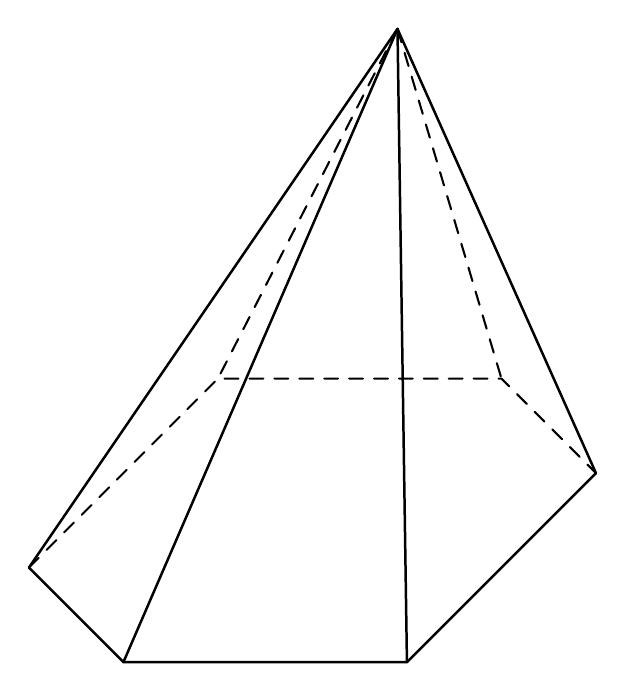
\begin{tikzpicture}[
    scale=1.2,
    line cap=round,
    line join=round,
    visible/.style={line width=0.9pt},
    hidden/.style={line width=0.75pt,dashed,dash pattern=on 5pt off 4pt}
]

% -------------------------------------------------
% Вершина пирамиды
% -------------------------------------------------
\coordinate (S) at (1.4,6.2);

% -------------------------------------------------
% Вершины правильноподобного шестиугольника в основании
% Расположены вручную по образцу рисунка
% -------------------------------------------------
\coordinate (A) at (-2.5,0.5);   % левая внешняя
\coordinate (B) at (-1.5,-0.5);  % левая передняя
\coordinate (C) at (1.5,-0.5);  % передняя центральная
\coordinate (D) at (3.5,1.5);  % правая передняя/внешняя
\coordinate (E) at (2.5,2.5);  % правая задняя
\coordinate (F) at (-0.5,2.5); % левая задняя

% -------------------------------------------------
% Основание
% -------------------------------------------------

% Видимые рёбра основания
\draw[visible] (A)--(B)--(C)--(D);

% Невидимые рёбра основания
\draw[hidden] (A)--(F)--(E)--(D);

% -------------------------------------------------
% Боковые рёбра
% -------------------------------------------------

% Видимые
\draw[visible] (S)--(A);
\draw[visible] (S)--(B);
\draw[visible] (S)--(C);
\draw[visible] (S)--(D);

% Невидимые
\draw[hidden] (S)--(F);
\draw[hidden] (S)--(E);

\end{tikzpicture}

\end{document}

Высота конуса равна 18, а длина образующей равна 30. Найдите площадь осевого сечения этого конуса.
\documentclass[tikz,border=4pt]{standalone}

\begin{document}

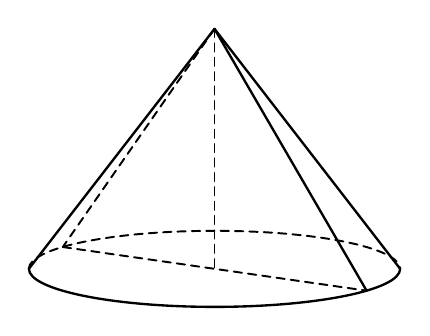
\begin{tikzpicture}[
    scale=1.15,
    line cap=round,
    line join=round,
    visible/.style={
        line width=0.85pt
    },
    hidden/.style={
        line width=0.7pt,
        dashed,
        dash pattern=on 3pt off 2.2pt
    }
]

% -------------------------------------------------
% Параметры изображения
% -------------------------------------------------

\def\R{2.05}    % горизонтальный радиус эллипса
\def\r{0.42}    % вертикальный радиус эллипса
\def\H{2.65}    % изображаемая высота конуса

% -------------------------------------------------
% Основные точки
% -------------------------------------------------

\coordinate (S) at (0,\H);   % вершина конуса
\coordinate (O) at (0,0);    % центр основания

% Крайние точки основания
\coordinate (L) at (-\R,0);
\coordinate (R) at ( \R,0);

% Концы диаметра осевого сечения
\coordinate (P) at
    ({(\R+1.3)*cos(120)},{\r*sin(145)});

\coordinate (Q) at
    ({\R*cos(-35)},{\r*sin(-35)});

% -------------------------------------------------
% Задняя половина основания
% -------------------------------------------------

\draw[hidden]
    (L)
    arc[
        start angle=180,
        end angle=0,
        x radius=\R,
        y radius=\r
    ];

% -------------------------------------------------
% Скрытая образующая осевого сечения
% -------------------------------------------------

\draw[hidden] (S)--(P);

% Диаметр основания в плоскости осевого сечения
\draw[hidden] (P)--(Q);

% Ось конуса
\draw[hidden] (S)--(O);

% -------------------------------------------------
% Внешние образующие конуса
% -------------------------------------------------

\draw[visible] (S)--(L);
\draw[visible] (S)--(R);

% Видимая образующая осевого сечения
\draw[visible] (S)--(Q);

% -------------------------------------------------
% Передняя половина основания
% -------------------------------------------------

\draw[visible]
    (R)
    arc[
        start angle=0,
        end angle=-180,
        x radius=\R,
        y radius=\r
    ];

\end{tikzpicture}

\end{document}

Диаметр основания конуса равен 32, а длина образующей равна 20. Найдите площадь осевого сечения этого конуса.
\documentclass[tikz,border=4pt]{standalone}

\begin{document}

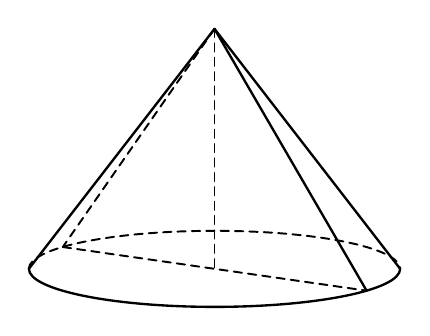
\begin{tikzpicture}[
    scale=1.15,
    line cap=round,
    line join=round,
    visible/.style={
        line width=0.85pt
    },
    hidden/.style={
        line width=0.7pt,
        dashed,
        dash pattern=on 3pt off 2.2pt
    }
]

% -------------------------------------------------
% Параметры изображения
% -------------------------------------------------

\def\R{2.05}    % горизонтальный радиус эллипса
\def\r{0.42}    % вертикальный радиус эллипса
\def\H{2.65}    % изображаемая высота конуса

% -------------------------------------------------
% Основные точки
% -------------------------------------------------

\coordinate (S) at (0,\H);   % вершина конуса
\coordinate (O) at (0,0);    % центр основания

% Крайние точки основания
\coordinate (L) at (-\R,0);
\coordinate (R) at ( \R,0);

% Концы диаметра осевого сечения
\coordinate (P) at
    ({(\R+1.3)*cos(120)},{\r*sin(145)});

\coordinate (Q) at
    ({\R*cos(-35)},{\r*sin(-35)});

% -------------------------------------------------
% Задняя половина основания
% -------------------------------------------------

\draw[hidden]
    (L)
    arc[
        start angle=180,
        end angle=0,
        x radius=\R,
        y radius=\r
    ];

% -------------------------------------------------
% Скрытая образующая осевого сечения
% -------------------------------------------------

\draw[hidden] (S)--(P);

% Диаметр основания в плоскости осевого сечения
\draw[hidden] (P)--(Q);

% Ось конуса
\draw[hidden] (S)--(O);

% -------------------------------------------------
% Внешние образующие конуса
% -------------------------------------------------

\draw[visible] (S)--(L);
\draw[visible] (S)--(R);

% Видимая образующая осевого сечения
\draw[visible] (S)--(Q);

% -------------------------------------------------
% Передняя половина основания
% -------------------------------------------------

\draw[visible]
    (R)
    arc[
        start angle=0,
        end angle=-180,
        x radius=\R,
        y radius=\r
    ];

\end{tikzpicture}

\end{document}

От треугольной призмы, объём которой равен 120, отсечена треугольная пирамида плоскостью, проходящей через сторону одного основания и противоположную вершину другого основания. Найдите объём оставшейся части.
\documentclass[tikz,border=4pt]{standalone}

\begin{document}

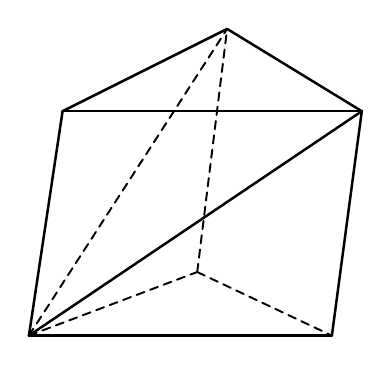
\begin{tikzpicture}[
    scale=0.95,
    line cap=round,
    line join=round,
    visible/.style={line width=0.9pt},
    hidden/.style={line width=0.7pt,dashed,dash pattern=on 3pt off 2.2pt}
]

% -------------------------------------------------
% Вершины
% Нижнее основание: A B C
% Верхнее основание: D E F
% -------------------------------------------------

\coordinate (A) at (0.20,0.20);   % нижняя левая передняя
\coordinate (B) at (2.45,1.05);   % нижняя дальняя
\coordinate (C) at (4.25,0.20);   % нижняя правая передняя

\coordinate (D) at (0.65,3.20);   % верхняя левая
\coordinate (E) at (2.85,4.30);   % верхняя вершина
\coordinate (F) at (4.65,3.20);   % верхняя правая 

% -------------------------------------------------
% Верхнее основание призмы
% -------------------------------------------------

\draw[visible] (D)--(E)--(F);
\draw[visible] (D)--(F);

% -------------------------------------------------
% Боковые рёбра призмы
% -------------------------------------------------

\draw[visible] (A)--(D);
\draw[hidden]  (B)--(E);
\draw[visible] (C)--(F);

% -------------------------------------------------
% Нижнее основание призмы
% -------------------------------------------------

\draw[visible] (A)--(C);
\draw[hidden]  (A)--(B);
\draw[hidden]  (B)--(C);

% -------------------------------------------------
% Линия сечения
% Плоскость проходит через сторону DF
% и противоположную вершину A
% -------------------------------------------------

\draw[visible] (A)--(F);
\draw[hidden] (A)--(E);
\end{tikzpicture}

\end{document}

Объём треугольной пирамиды равен 14. Плоскость проходит через сторону основания этой пирамиды и пересекает противоположное боковое ребро в точке, делящей его в отношении 2:5, считая от вершины пирамиды. Найдите большую из объёмов пирамид, на которые плоскость разбивает исходную пирамиду.
\documentclass[tikz,border=4pt]{standalone}

\usetikzlibrary{calc}

\begin{document}

\begin{tikzpicture}[
    scale=0.95,
    line cap=round,
    line join=round,
    visible/.style={line width=0.9pt},
    hidden/.style={line width=0.7pt,dashed,dash pattern=on 3pt off 2.2pt}
]

% -------------------------------------------------
% Вершины пирамиды
% -------------------------------------------------

\coordinate (S) at (2.20,4.90);   % вершина
\coordinate (A) at (0.85,1.65);   % левая вершина основания
\coordinate (B) at (1.65,0.15);   % передняя вершина основания
\coordinate (C) at (4.95,1.05);   % правая вершина основания

% Точка на противоположном боковом ребре SC
% Делит его в отношении 2:5 от вершины S
\coordinate (P) at ($(S)!2/7!(C)$);

% -------------------------------------------------
% Основание
% -------------------------------------------------

\draw[visible] (A)--(B)--(C);
\draw[hidden]  (A)--(C);

% -------------------------------------------------
% Боковые рёбра
% -------------------------------------------------

\draw[visible] (S)--(A);
\draw[visible] (S)--(B);
\draw[visible] (S)--(C);

% -------------------------------------------------
% Сечение плоскостью через сторону AB
% и точку P на ребре SC
% -------------------------------------------------

\draw[hidden]  (A)--(P);
\draw[visible] (B)--(P);

\end{tikzpicture}

\end{document}

Из единичного куба вырезана правильная четырёхугольная призма со стороной основания 0{,}4 и боковым ребром 1. Найдите площадь поверхности оставшейся части куба.
\documentclass[tikz,border=4pt]{standalone}

\begin{document}

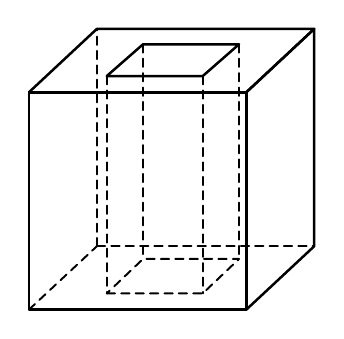
\begin{tikzpicture}[
    scale=1.15,
    line cap=round,
    line join=round,
    visible/.style={
        line width=0.9pt
    },
    hidden/.style={
        line width=0.7pt,
        dashed,
        dash pattern=on 3pt off 2.2pt
    }
]

% =================================================
% Вершины куба
% =================================================

% Передняя грань
\coordinate (A) at (0,0);
\coordinate (B) at (2.4,0);
\coordinate (C) at (2.4,2.4);
\coordinate (D) at (0,2.4);

% Задняя грань
\coordinate (A1) at (0.75,0.70);
\coordinate (B1) at (3.15,0.70);
\coordinate (C1) at (3.15,3.10);
\coordinate (D1) at (0.75,3.10);

% =================================================
% Верхнее основание вырезанной призмы
% =================================================

\coordinate (P1) at (0.86,2.58);
\coordinate (P2) at (1.92,2.58);
\coordinate (P3) at (2.32,2.93);
\coordinate (P4) at (1.26,2.93);

% Нижнее основание вырезанной призмы
\coordinate (Q1) at (0.86,0.18);
\coordinate (Q2) at (1.92,0.18);
\coordinate (Q3) at (2.32,0.56);
\coordinate (Q4) at (1.26,0.56);

% =================================================
% Скрытые рёбра куба
% =================================================

\draw[hidden] (A)--(A1);
\draw[hidden] (A1)--(B1);
\draw[hidden] (A1)--(D1);

% =================================================
% Внутренние рёбра отверстия
% =================================================

% Вертикальные рёбра вырезанной призмы
\draw[hidden] (P1)--(Q1);
\draw[hidden] (P2)--(Q2);
\draw[hidden] (P3)--(Q3);
\draw[hidden] (P4)--(Q4);

% Нижнее основание отверстия
\draw[hidden]
    (Q1)--(Q2)--(Q3)--(Q4)--cycle;

% =================================================
% Видимые рёбра куба
% =================================================

% Передняя грань
\draw[visible]
    (A)--(B)--(C)--(D)--cycle;

% Верхняя грань
\draw[visible]
    (D)--(D1)--(C1)--(C);

% Правая грань
\draw[visible]
    (C)--(C1)--(B1)--(B);

% =================================================
% Верхний край отверстия
% =================================================

\draw[visible]
    (P1)--(P2)--(P3)--(P4)--cycle;

\end{tikzpicture}

\end{document}

Из единичного куба вырезана правильная четырёхугольная призма со стороной основания 0{,}6 и боковым ребром 1. Найдите площадь поверхности оставшейся части куба.
\documentclass[tikz,border=4pt]{standalone}

\begin{document}

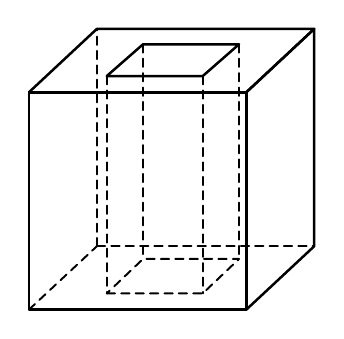
\begin{tikzpicture}[
    scale=1.15,
    line cap=round,
    line join=round,
    visible/.style={
        line width=0.9pt
    },
    hidden/.style={
        line width=0.7pt,
        dashed,
        dash pattern=on 3pt off 2.2pt
    }
]

% =================================================
% Вершины куба
% =================================================

% Передняя грань
\coordinate (A) at (0,0);
\coordinate (B) at (2.4,0);
\coordinate (C) at (2.4,2.4);
\coordinate (D) at (0,2.4);

% Задняя грань
\coordinate (A1) at (0.75,0.70);
\coordinate (B1) at (3.15,0.70);
\coordinate (C1) at (3.15,3.10);
\coordinate (D1) at (0.75,3.10);

% =================================================
% Верхнее основание вырезанной призмы
% =================================================

\coordinate (P1) at (0.86,2.58);
\coordinate (P2) at (1.92,2.58);
\coordinate (P3) at (2.32,2.93);
\coordinate (P4) at (1.26,2.93);

% Нижнее основание вырезанной призмы
\coordinate (Q1) at (0.86,0.18);
\coordinate (Q2) at (1.92,0.18);
\coordinate (Q3) at (2.32,0.56);
\coordinate (Q4) at (1.26,0.56);

% =================================================
% Скрытые рёбра куба
% =================================================

\draw[hidden] (A)--(A1);
\draw[hidden] (A1)--(B1);
\draw[hidden] (A1)--(D1);

% =================================================
% Внутренние рёбра отверстия
% =================================================

% Вертикальные рёбра вырезанной призмы
\draw[hidden] (P1)--(Q1);
\draw[hidden] (P2)--(Q2);
\draw[hidden] (P3)--(Q3);
\draw[hidden] (P4)--(Q4);

% Нижнее основание отверстия
\draw[hidden]
    (Q1)--(Q2)--(Q3)--(Q4)--cycle;

% =================================================
% Видимые рёбра куба
% =================================================

% Передняя грань
\draw[visible]
    (A)--(B)--(C)--(D)--cycle;

% Верхняя грань
\draw[visible]
    (D)--(D1)--(C1)--(C);

% Правая грань
\draw[visible]
    (C)--(C1)--(B1)--(B);

% =================================================
% Верхний край отверстия
% =================================================

\draw[visible]
    (P1)--(P2)--(P3)--(P4)--cycle;

\end{tikzpicture}

\end{document}

В кубе ABCDA_1B_1C_1D_1 найдите угол между прямыми DC_1 и BD. Ответ дайте в градусах.
\documentclass[tikz,border=4pt]{standalone}

\begin{document}

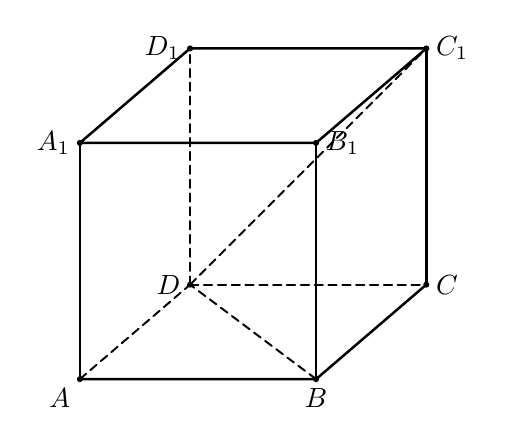
\begin{tikzpicture}[
    scale=1,
    line cap=round,
    line join=round,
    visible/.style={line width=0.9pt},
    hidden/.style={line width=0.7pt,dashed,dash pattern=on 3pt off 2pt}
]

% -------------------------------------------------
% Вершины куба
% Нижнее основание: ABCD
% Верхнее основание: A1B1C1D1
% -------------------------------------------------

\coordinate (A)  at (0,0);
\coordinate (B)  at (3,0);
\coordinate (C)  at (4.4,1.2);
\coordinate (D)  at (1.4,1.2);

\coordinate (A1) at (0,3);
\coordinate (B1) at (3,3);
\coordinate (C1) at (4.4,4.2);
\coordinate (D1) at (1.4,4.2);

% -------------------------------------------------
% Скрытые рёбра куба
% -------------------------------------------------

\draw[hidden] (A)--(D);
\draw[hidden] (D)--(C);
\draw[hidden] (D)--(D1);

% -------------------------------------------------
% Видимые рёбра куба
% -------------------------------------------------

\draw[visible] (A)--(B)--(C);
\draw[visible] (A)--(A1);
\draw[visible] (B)--(B1);
\draw[visible] (C)--(C1);

\draw[visible] (A1)--(B1)--(C1)--(D1)--cycle;
\draw[visible] (C1)--(C);

% -------------------------------------------------
% Нужные прямые
% -------------------------------------------------

% Диагональ основания BD
\draw[hidden] (B)--(D);

% Прямая DC1
\draw[hidden] (D)--(C1);

% -------------------------------------------------
% Подписи вершин
% -------------------------------------------------

\fill (A)  circle (1.1pt) node[below left]  {$A$};
\fill (B)  circle (1.1pt) node[below]       {$B$};
\fill (C)  circle (1.1pt) node[right]       {$C$};
\fill (D)  circle (1.1pt) node[left]        {$D$};

\fill (A1) circle (1.1pt) node[left]        {$A_1$};
\fill (B1) circle (1.1pt) node[right]       {$B_1$};
\fill (C1) circle (1.1pt) node[right]       {$C_1$};
\fill (D1) circle (1.1pt) node[left]        {$D_1$};

\end{tikzpicture}

\end{document}

В правильной треугольной призме ABCA_1B_1C_1, все рёбра которой равны 2, найдите угол между прямыми BB_1 и AC_1. Ответ дайте в градусах.
\documentclass[tikz,border=4pt]{standalone}

\begin{document}

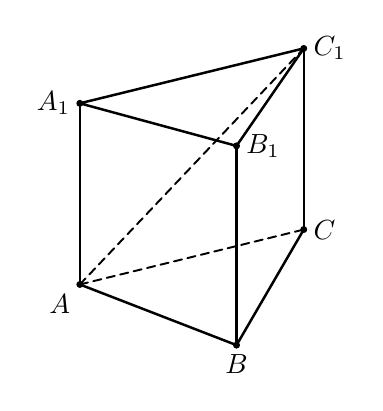
\begin{tikzpicture}[
    x={(1cm,0cm)},
    y={(0.85cm,0.35cm)},
    z={(0cm,1cm)},
    scale=1.15,
    line cap=round,
    line join=round,
    visible/.style={line width=0.9pt},
    hidden/.style={line width=0.7pt,dashed,dash pattern=on 3pt off 2pt}
]

% -------------------------------------------------
% Вершины призмы
% Нижнее основание ABC
% Верхнее основание A1B1C1
% Все рёбра равны 2
% -------------------------------------------------

\coordinate (A)  at (0,0,0);
\coordinate (B)  at (1.9,-0.2,-0.6);
\coordinate (C)  at (1,{sqrt(3)},0);

\coordinate (A1) at (0,0,2);
\coordinate (B1) at (1.9,-0.2,1.6);
\coordinate (C1) at (1,{sqrt(3)},2);

% -------------------------------------------------
% Основания призмы
% -------------------------------------------------


\draw[hidden] (A)--(C);
\draw[visible] (B)--(C);
\draw[visible] (B)--(A);
\draw[visible] (A1)--(B1)--(C1)--cycle;

% -------------------------------------------------
% Боковые рёбра
% -------------------------------------------------

\draw[visible] (A)--(A1);
\draw[visible] (B)--(B1);
\draw[visible] (C)--(C1);

% -------------------------------------------------
% Нужные прямые
% -------------------------------------------------

% BB1 уже является боковым ребром
\draw[hidden] (A)--(C1);

% -------------------------------------------------
% Подписи вершин
% -------------------------------------------------

\fill (A)  circle (1.1pt) node[below left]  {$A$};
\fill (B)  circle (1.1pt) node[below]       {$B$};
\fill (C)  circle (1.1pt) node[right]       {$C$};

\fill (A1) circle (1.1pt) node[left]        {$A_1$};
\fill (B1) circle (1.1pt) node[right]       {$B_1$};
\fill (C1) circle (1.1pt) node[right]       {$C_1$};

\end{tikzpicture}

\end{document}

Радиусы двух шаров равны 7 и 24. Найдите радиус шара, площадь поверхности которого равна сумме площадей поверхностей двух данных шаров.
\documentclass[tikz,border=4pt]{standalone}
 \usetikzlibrary{calc}
\begin{document}

\begin{tikzpicture}[
    scale=0.9,
    line cap=round,
    line join=round,
    sphere/.style={line width=0.9pt},
    hidden/.style={
        line width=0.65pt,
        dashed,
        dash pattern=on 3pt off 2pt
    },
    label/.style={font=\small}
]

% =================================================
% Первый шар
% =================================================

\coordinate (O1) at (0,0);
\def\rone{1.15}

% Контур шара
\draw[sphere] (O1) circle[radius=\rone];

% Экватор
\draw[hidden]
    ($(O1)+(-\rone,0)$)
    arc[
        start angle=180,
        end angle=0,
        x radius=\rone,
        y radius=0.28
    ];

\draw[sphere]
    ($(O1)+(\rone,0)$)
    arc[
        start angle=0,
        end angle=-180,
        x radius=\rone,
        y radius=0.28
    ];

% Радиус
\draw[sphere] (O1)--++(35:\rone);

\fill (O1) circle (1.1pt);


% =================================================
% Второй шар
% =================================================

\coordinate (O2) at (3.8,0);
\def\rtwo{1.75}

% Контур шара
\draw[sphere] (O2) circle[radius=\rtwo];

% Экватор
\draw[hidden]
    ($(O2)+(-\rtwo,0)$)
    arc[
        start angle=180,
        end angle=0,
        x radius=\rtwo,
        y radius=0.42
    ];

\draw[sphere]
    ($(O2)+(\rtwo,0)$)
    arc[
        start angle=0,
        end angle=-180,
        x radius=\rtwo,
        y radius=0.42
    ];

% Радиус
\draw[sphere] (O2)--++(35:\rtwo);

\fill (O2) circle (1.1pt);


\end{tikzpicture}

\end{document}

Объём параллелепипеда ABCDA_1B_1C_1D_1 равен 60. Найдите объём треугольной пирамиды ACB_1D_1.
\documentclass[tikz,border=4pt]{standalone}

\begin{document}

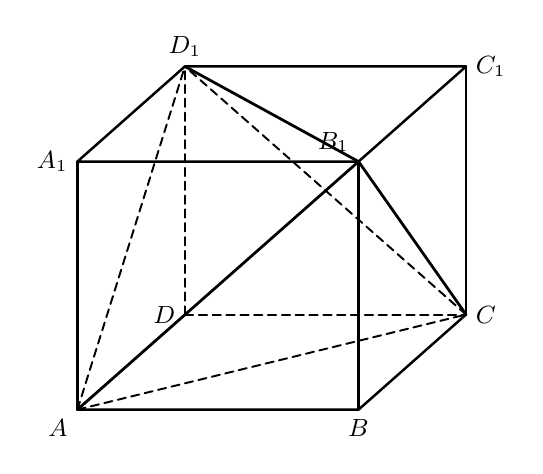
\begin{tikzpicture}[
    scale=1.05,
    line cap=round,
    line join=round,
    edge/.style={
        line width=0.9pt
    },
    hidden/.style={
        line width=0.7pt,
        dashed,
        dash pattern=on 3pt off 2pt
    },
    section/.style={
        line width=1pt
    },
    every node/.style={
        font=\small
    }
]

% =================================================
% Вершины параллелепипеда
% =================================================

% Нижнее основание ABCD
\coordinate (A) at (0,0);
\coordinate (B) at (3.4,0);
\coordinate (C) at (4.7,1.15);
\coordinate (D) at (1.3,1.15);

% Верхнее основание A_1B_1C_1D_1
\coordinate (A1) at (0,3);
\coordinate (B1) at (3.4,3);
\coordinate (C1) at (4.7,4.15);
\coordinate (D1) at (1.3,4.15);

% =================================================
% Скрытые рёбра параллелепипеда
% =================================================

\draw[hidden] (A)--(D);
\draw[hidden] (D)--(C);
\draw[hidden] (D)--(D1);

% =================================================
% Видимые рёбра параллелепипеда
% =================================================

\draw[edge] (A)--(B)--(C);
\draw[edge] (A)--(A1);
\draw[edge] (B)--(B1);
\draw[edge] (C)--(C1);

\draw[edge]
    (A1)--(B1)--(C1)--(D1)--cycle;

% =================================================
% Рёбра пирамиды ACB_1D_1
% =================================================

% Ребро AC лежит в нижнем основании
\draw[hidden] (A)--(C);

% Рёбра, соединяющие нижние и верхние вершины
\draw[section] (A)--(B1);
\draw[hidden]  (A)--(D1);

\draw[section] (C)--(B1);
\draw[hidden] (C)--(D1);

% Ребро B_1D_1 лежит в верхнем основании
\draw[section] (B1)--(D1);

% =================================================
% Подписи
% =================================================

\node[below left]  at (A)  {$A$};
\node[below]       at (B)  {$B$};
\node[right]       at (C)  {$C$};
\node[left]        at (D)  {$D$};

\node[left]        at (A1) {$A_1$};
\node[above left]  at (B1) {$B_1$};
\node[right]       at (C1) {$C_1$};
\node[above]       at (D1) {$D_1$};

\end{tikzpicture}

\end{document}

В прямоугольном параллелепипеде ABCDA_1B_1C_1D_1 известно, что AB=9, BC=6, AA_1=5. Найдите объём многогранника, вершинами которого являются точки A, B, C, D, A_1, B_1.
\documentclass[tikz,border=4pt]{standalone}

\begin{document}

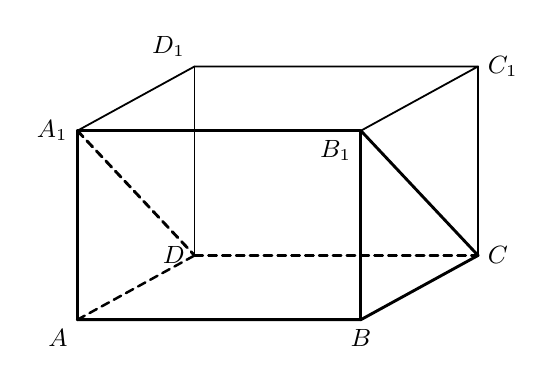
\begin{tikzpicture}[
    x={(1cm,0cm)},
    y={(0.62cm,0.34cm)},
    z={(0cm,1cm)},
    scale=0.8,
    line cap=round,
    line join=round,
    cube/.style={
        line width=0.65pt
    },
    hidden/.style={
        line width=0.65pt,
        dashed,
        dash pattern=on 3pt off 2pt
    },
    solid/.style={
        line width=1.05pt
    },
    solidhidden/.style={
        line width=0.9pt,
        dashed,
        dash pattern=on 3pt off 2pt
    },
    every node/.style={
        font=\small
    }
]

% =================================================
% Вершины прямоугольного параллелепипеда
% =================================================

\coordinate (A)  at (0,0,0);
\coordinate (B)  at (4.5,0,0);
\coordinate (C)  at (4.5,3,0);
\coordinate (D)  at (0,3,0);

\coordinate (A1) at (0,0,3);
\coordinate (B1) at (4.5,0,3);
\coordinate (C1) at (4.5,3,3);
\coordinate (D1) at (0,3,3);

% =================================================
% Рёбра исходного параллелепипеда,
% которые не входят в искомый многогранник
% =================================================

\draw[cube] (A1)--(D1)--(C1)--(B1);
\draw[cube] (D1)--(D);
\draw[cube] (C1)--(C);

% =================================================
% Скрытые рёбра искомого многогранника
% =================================================

\draw[solidhidden] (A)--(D);
\draw[solidhidden] (D)--(C);

% =================================================
% Видимые рёбра искомого многогранника
% =================================================

% Нижняя грань ABCD
\draw[solid] (A)--(B)--(C);

% Прямоугольная грань ABB_1A_1
\draw[solid] (A)--(A1)--(B1)--(B);

% Наклонная грань A_1B_1CD
\draw[hidden,solid] (A1)--(D);
\draw[solid] (B1)--(C);

% =================================================
% Подписи вершин
% =================================================

\node[below left]  at (A)  {$A$};
\node[below]       at (B)  {$B$};
\node[right]       at (C)  {$C$};
\node[left]        at (D)  {$D$};

\node[left]        at (A1) {$A_1$};
\node[below left] at (B1) {$B_1$};
\node[right]       at (C1) {$C_1$};
\node[above left]  at (D1) {$D_1$};

\end{tikzpicture}

\end{document}

В прямоугольном параллелепипеде ABCDA_1B_1C_1D_1 известно, что AB=9, BC=8, AA_1=6. Найдите объём многогранника, вершинами которого являются точки A, B, C, B_1.
\documentclass[tikz,border=4pt]{standalone}

\begin{document}

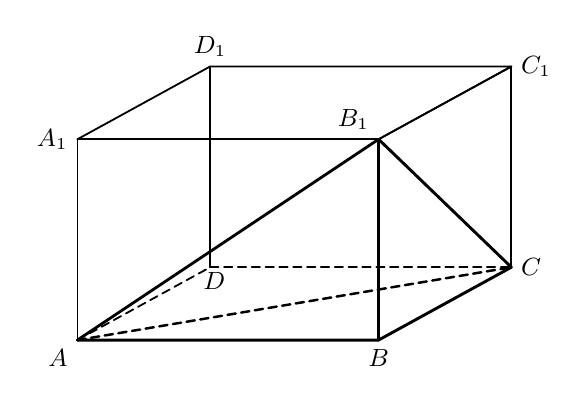
\begin{tikzpicture}[
    x={(1cm,0cm)},
    y={(0.62cm,0.34cm)},
    z={(0cm,1cm)},
    scale=0.85,
    line cap=round,
    line join=round,
    boxedge/.style={
        line width=0.65pt
    },
    hidden/.style={
        line width=0.65pt,
        dashed,
        dash pattern=on 3pt off 2pt
    },
    solid/.style={
        line width=1.05pt
    },
    solidhidden/.style={
        line width=0.9pt,
        dashed,
        dash pattern=on 3pt off 2pt
    },
    every node/.style={
        font=\small
    }
]

% =================================================
% Вершины прямоугольного параллелепипеда
% =================================================

\coordinate (A)  at (0,0,0);
\coordinate (B)  at (4.5,0,0);
\coordinate (C)  at (4.5,3.2,0);
\coordinate (D)  at (0,3.2,0);

\coordinate (A1) at (0,0,3);
\coordinate (B1) at (4.5,0,3);
\coordinate (C1) at (4.5,3.2,3);
\coordinate (D1) at (0,3.2,3);

% =================================================
% Скрытые рёбра параллелепипеда
% =================================================

\draw[hidden] (A)--(D);
\draw[hidden] (D)--(C);
\draw[hidden] (D)--(D1);

% =================================================
% Видимые рёбра параллелепипеда
% =================================================

\draw[boxedge] (A)--(A1)--(B1);
\draw[boxedge] (A1)--(D1)--(C1)--(B1);
\draw[boxedge] (D1)--(D);
\draw[boxedge] (C1)--(C);
\draw[boxedge] (B1)--(C1);

% =================================================
% Рёбра пирамиды ABCB_1
% =================================================

% Рёбра основания ABC
\draw[solid]       (A)--(B)--(C);
\draw[solidhidden] (A)--(C);

% Боковые рёбра
\draw[solid] (A)--(B1);
\draw[solid] (B)--(B1);
\draw[solid] (C)--(B1);

% =================================================
% Подписи вершин
% =================================================

\node[below left]  at (A)  {$A$};
\node[below]       at (B)  {$B$};
\node[right]       at (C)  {$C$};
\node[right, xshift=-6pt, yshift=-5pt] at (D) {$D$};

\node[left]        at (A1) {$A_1$};
\node[above left]  at (B1) {$B_1$};
\node[right]       at (C1) {$C_1$};
\node[above]       at (D1) {$D_1$};

\end{tikzpicture}

\end{document}

\section*{Вариант 17}

В сосуде, имеющем форму конуса, уровень жидкости достигает
\(0{,}25\) высоты. Объём жидкости равен \(5\) мл.
Сколько миллилитров жидкости нужно долить, чтобы полностью
наполнить сосуд?

\begin{center}
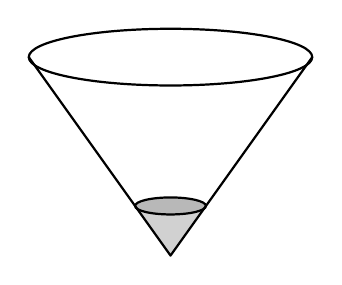
\begin{tikzpicture}[
  scale=0.9,
  line cap=round,
  line join=round
]
  \coordinate (S) at (0,-2.8);
  \coordinate (L) at (-2,0);
  \coordinate (R) at (2,0);

  % Точки на уровне жидкости:
  % высота малого конуса составляет 0,25 высоты большого
  \coordinate (A) at (-0.5,-2.1);
  \coordinate (B) at (0.5,-2.1);

  % Жидкость
  \fill[black!18]
    (S) --
    (A)
    arc[
      start angle=180,
      end angle=360,
      x radius=0.5,
      y radius=0.12
    ]
    -- cycle;

  \fill[black!28]
    (0,-2.1)
    ellipse[
      x radius=0.5,
      y radius=0.12
    ];

  % Сосуд
  \draw[thick]
    (0,0)
    ellipse[
      x radius=2,
      y radius=0.4
    ];

  \draw[thick]
    (L) -- (S) -- (R);

  % Поверхность жидкости
  \draw[thick]
    (0,-2.1)
    ellipse[
      x radius=0.5,
      y radius=0.12
    ];
\end{tikzpicture}
\end{center}
\section*{Вариант 18}

В сосуд, имеющий форму правильной треугольной призмы, налили
\(1100\) см\(^{3}\) воды и полностью в неё погрузили деталь.
При этом уровень жидкости в сосуде поднялся с отметки \(25\) см
до отметки \(29\) см. Чему равен объём детали?
Ответ выразите в см\(^{3}\).

\begin{center}
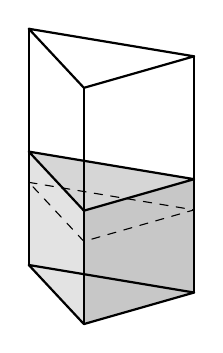
\begin{tikzpicture}[
  scale=1,
  line cap=round,
  line join=round
]
  % Верхнее основание призмы
  \coordinate (A) at (-0.9,2.7);
  \coordinate (B) at (1.2,2.35);
  \coordinate (C) at (-0.2,1.95);

  % Нижнее основание призмы
  \coordinate (A1) at (-0.9,-0.3);
  \coordinate (B1) at (1.2,-0.65);
  \coordinate (C1) at (-0.2,-1.05);

  % Новый уровень жидкости — 29 см
  \coordinate (A29) at (-0.9,1.14);
  \coordinate (B29) at (1.2,0.79);
  \coordinate (C29) at (-0.2,0.39);

  % Первоначальный уровень жидкости — 25 см
  \coordinate (A25) at (-0.9,0.75);
  \coordinate (B25) at (1.2,0.40);
  \coordinate (C25) at (-0.2,0);

  % Жидкость после погружения детали
  \fill[black!16]
    (A1) -- (B1) -- (B29) -- (A29) -- cycle;

  \fill[black!22]
    (B1) -- (C1) -- (C29) -- (B29) -- cycle;

  \fill[black!11]
    (C1) -- (A1) -- (A29) -- (C29) -- cycle;





  % Рёбра призмы
  \draw[thick]
    (A) -- (B) -- (C) -- cycle;

  \draw[thick] (A) -- (A1);
  \draw[thick] (B) -- (B1);
  \draw[thick] (C) -- (C1);

  \draw[thick]
    (A1) -- (B1) -- (C1) -- cycle;

  % Уровень до погружения детали
  \draw[dashed]
    (A25) -- (B25) -- (C25) -- cycle;

  % Уровень после погружения детали
  \draw[thick]
    (A29) -- (B29) -- (C29) -- cycle;
\end{tikzpicture}
\end{center}

\section*{Вариант 19}

Дано два цилиндра. Объём первого цилиндра равен \(5\).
У второго цилиндра высота в \(2{,}5\) раза меньше,
а радиус основания в \(3\) раза больше, чем у первого.
Найдите объём второго цилиндра.

\begin{center}
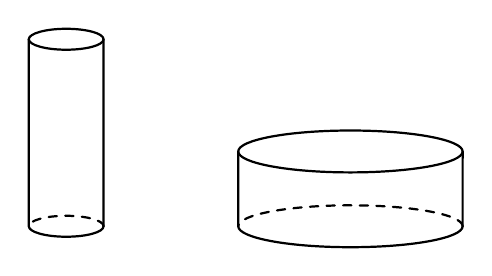
\begin{tikzpicture}[
  scale=0.95,
  line cap=round,
  line join=round
]
  % Первый цилиндр:
  % r_1 = 0.5, h_1 = 2.5
  \coordinate (L1) at (-0.5,0);
  \coordinate (R1) at (0.5,0);

  \draw[thick]
    (0,2.5) ellipse[x radius=0.5,y radius=0.14];

  \draw[thick]
    (L1) -- (-0.5,2.5);

  \draw[thick]
    (R1) -- (0.5,2.5);

  % Передняя и задняя части нижнего основания
  \draw[thick]
    (-0.5,0)
    arc[
      start angle=180,
      end angle=360,
      x radius=0.5,
      y radius=0.14
    ];

  \draw[thick,dashed]
    (0.5,0)
    arc[
      start angle=0,
      end angle=180,
      x radius=0.5,
      y radius=0.14
    ];

  % Второй цилиндр:
  % r_2 = 3r_1 = 1.5,
  % h_2 = h_1/2.5 = 1
  \coordinate (L2) at (2.3,0);
  \coordinate (R2) at (5.3,0);

  \draw[thick]
    (3.8,1)
    ellipse[x radius=1.5,y radius=0.28];

  \draw[thick]
    (L2) -- (2.3,1);

  \draw[thick]
    (R2) -- (5.3,1);

  % Передняя и задняя части нижнего основания
  \draw[thick]
    (2.3,0)
    arc[
      start angle=180,
      end angle=360,
      x radius=1.5,
      y radius=0.28
    ];

  \draw[thick,dashed]
    (5.3,0)
    arc[
      start angle=0,
      end angle=180,
      x radius=1.5,
      y radius=0.28
    ];
\end{tikzpicture}
\end{center}
\section*{Вариант 20}

В цилиндрическом сосуде уровень жидкости достигает \(25\) см.
На какой высоте будет находиться уровень жидкости, если её перелить
во второй цилиндрический сосуд, диаметр которого в \(2{,}5\) раза
больше диаметра первого?

Ответ дайте в сантиметрах.

\begin{center}
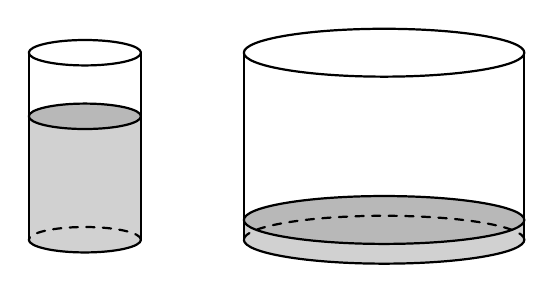
\begin{tikzpicture}[
  scale=0.95,
  line cap=round,
  line join=round
]
  % Первый сосуд
  \def\rone{0.75}
  \def\hone{2.5}
  \def\waterone{1.65}

  % Жидкость
  \fill[black!18]
    (-\rone,0) rectangle (\rone,\waterone);

  \fill[black!18]
    (0,0)
    ellipse[x radius=\rone,y radius=0.17];

  \fill[black!28]
    (0,\waterone)
    ellipse[x radius=\rone,y radius=0.17];

  % Стенки сосуда
  \draw[thick]
    (0,\hone)
    ellipse[x radius=\rone,y radius=0.17];

  \draw[thick]
    (-\rone,0) -- (-\rone,\hone);

  \draw[thick]
    (\rone,0) -- (\rone,\hone);

  \draw[thick]
    (-\rone,0)
    arc[
      start angle=180,
      end angle=360,
      x radius=\rone,
      y radius=0.17
    ];

  \draw[thick,dashed]
    (\rone,0)
    arc[
      start angle=0,
      end angle=180,
      x radius=\rone,
      y radius=0.17
    ];

  \draw[thick]
    (0,\waterone)
    ellipse[x radius=\rone,y radius=0.17];

  % Второй сосуд:
  % диаметр и радиус в 2.5 раза больше,
  % поэтому уровень жидкости значительно ниже
  \begin{scope}[xshift=4cm]
    \def\rtwo{1.875}
    \def\htwo{2.5}
    \def\watertwo{0.264}

    % Жидкость
    \fill[black!18]
      (-\rtwo,0) rectangle (\rtwo,\watertwo);

    \fill[black!18]
      (0,0)
      ellipse[x radius=\rtwo,y radius=0.32];

    \fill[black!28]
      (0,\watertwo)
      ellipse[x radius=\rtwo,y radius=0.32];

    % Стенки сосуда
    \draw[thick]
      (0,\htwo)
      ellipse[x radius=\rtwo,y radius=0.32];

    \draw[thick]
      (-\rtwo,0) -- (-\rtwo,\htwo);

    \draw[thick]
      (\rtwo,0) -- (\rtwo,\htwo);

    \draw[thick]
      (-\rtwo,0)
      arc[
        start angle=180,
        end angle=360,
        x radius=\rtwo,
        y radius=0.32
      ];

    \draw[thick,dashed]
      (\rtwo,0)
      arc[
        start angle=0,
        end angle=180,
        x radius=\rtwo,
        y radius=0.32
      ];

    \draw[thick]
      (0,\watertwo)
      ellipse[x radius=\rtwo,y radius=0.32];
  \end{scope}
\end{tikzpicture}
\end{center}
\section*{Вариант 21}

Цилиндр и конус имеют общие основание и высоту.
Объём цилиндра равен \(162\).
Найдите объём конуса.

\begin{center}
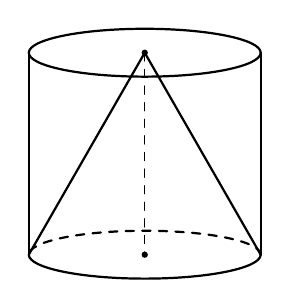
\begin{tikzpicture}[
  scale=0.95,
  line cap=round,
  line join=round
]
  \def\radius{1.55}
  \def\height{2.7}
  \def\ellipseheight{0.32}

  \coordinate (S) at (0,\height);
  \coordinate (L) at (-\radius,0);
  \coordinate (R) at (\radius,0);
  \coordinate (O) at (0,0);

  % Верхнее основание цилиндра
  \draw[thick]
    (0,\height)
    ellipse[
      x radius=\radius,
      y radius=\ellipseheight
    ];

  % Боковые рёбра цилиндра
  \draw[thick]
    (-\radius,0) -- (-\radius,\height);

  \draw[thick]
    (\radius,0) -- (\radius,\height);

  % Нижнее основание цилиндра
  \draw[thick]
    (L)
    arc[
      start angle=180,
      end angle=360,
      x radius=\radius,
      y radius=\ellipseheight
    ];

  \draw[thick,dashed]
    (R)
    arc[
      start angle=0,
      end angle=180,
      x radius=\radius,
      y radius=\ellipseheight
    ];

  % Конус
  \draw[thick]
    (S) -- (L);

  \draw[thick]
    (S) -- (R);

  % Высота конуса
  \draw[dashed]
    (S) -- (O);

  \fill (S) circle (1.2pt);
  \fill (O) circle (1.2pt);
\end{tikzpicture}
\end{center}
\section*{Вариант 22}

Цилиндр и конус имеют общие основание и высоту.
Высота цилиндра равна радиусу основания.
Площадь боковой поверхности цилиндра равна \(27\sqrt{2}\).
Найдите площадь боковой поверхности конуса.

\begin{center}
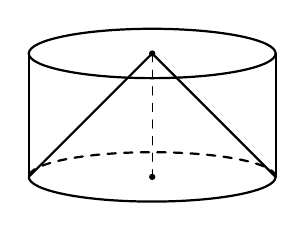
\begin{tikzpicture}[
  scale=0.95,
  line cap=round,
  line join=round
]
  % Высота цилиндра визуально равна радиусу основания
  \def\radius{1.65}
  \def\height{1.65}
  \def\ellipseheight{0.33}

  \coordinate (S) at (0,\height);
  \coordinate (L) at (-\radius,0);
  \coordinate (R) at (\radius,0);
  \coordinate (O) at (0,0);

  % Верхнее основание цилиндра
  \draw[thick]
    (0,\height)
    ellipse[
      x radius=\radius,
      y radius=\ellipseheight
    ];

  % Боковые рёбра цилиндра
  \draw[thick]
    (-\radius,0) -- (-\radius,\height);

  \draw[thick]
    (\radius,0) -- (\radius,\height);

  % Нижнее основание цилиндра
  \draw[thick]
    (L)
    arc[
      start angle=180,
      end angle=360,
      x radius=\radius,
      y radius=\ellipseheight
    ];

  \draw[thick,dashed]
    (R)
    arc[
      start angle=0,
      end angle=180,
      x radius=\radius,
      y radius=\ellipseheight
    ];

  % Конус с теми же основанием и высотой
  \draw[thick]
    (S) -- (L);

  \draw[thick]
    (S) -- (R);

  % Высота конуса
  \draw[dashed]
    (S) -- (O);

  \fill (S) circle (1.2pt);
  \fill (O) circle (1.2pt);
\end{tikzpicture}
\end{center}

\section*{Вариант 23}

\textbf{5.} Конус вписан в шар. Радиус основания конуса равен радиусу шара.
Объём шара равен \(188\). Найдите объём конуса.

\begin{center}
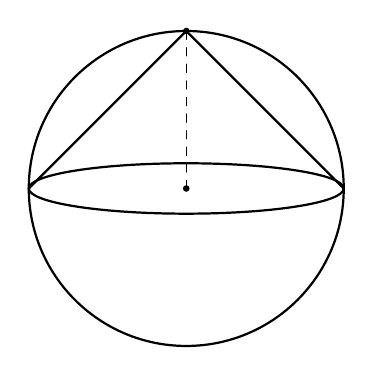
\begin{tikzpicture}[
  scale=1,
  line cap=round,
  line join=round
]
  \def\R{2}
  \def\ey{0.32}

  \coordinate (O) at (0,0);
  \coordinate (S) at (0,2);
  \coordinate (A) at (-2,0);
  \coordinate (B) at (2,0);

  % Шар
  \draw[thick] (O) circle (\R);

  % Основание конуса
  \draw[thick] (B) arc[start angle=0,end angle=180,x radius=2,y radius=\ey];
  \draw[thick] (A) arc[start angle=180,end angle=360,x radius=2,y radius=\ey];

  % Образующие конуса
  \draw[thick] (S)--(A);
  \draw[thick] (S)--(B);

  % Ось
  \draw[dashed] (S)--(O);

  \fill (S) circle (1.2pt);
  \fill (O) circle (1.2pt);
\end{tikzpicture}
\end{center}
\section*{Вариант 24}

\textbf{5.} Конус вписан в шар. Радиус основания конуса равен радиусу шара.
Объём конуса равен \(19\). Найдите объём шара.

\begin{center}
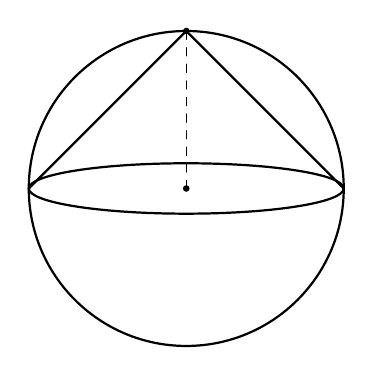
\begin{tikzpicture}[
  scale=1,
  line cap=round,
  line join=round
]
  \def\R{2}
  \def\ey{0.32}

  \coordinate (O) at (0,0);
  \coordinate (S) at (0,2);
  \coordinate (A) at (-2,0);
  \coordinate (B) at (2,0);

  % Шар
  \draw[thick] (O) circle (\R);

  % Основание конуса
  \draw[thick] (B) arc[start angle=0,end angle=180,x radius=2,y radius=\ey];
  \draw[thick] (A) arc[start angle=180,end angle=360,x radius=2,y radius=\ey];

  % Образующие конуса
  \draw[thick] (S)--(A);
  \draw[thick] (S)--(B);

  % Ось
  \draw[dashed] (S)--(O);

  \fill (S) circle (1.2pt);
  \fill (O) circle (1.2pt);
\end{tikzpicture}
\end{center}
\section*{Вариант 25}

\textbf{5.} Объём треугольной призмы, отсекаемой от куба плоскостью,
проходящей через середины двух рёбер, выходящих из одной вершины,
и параллельной третьему ребру, выходящему из этой же вершины,
равен \(25\). Найдите объём куба.

\begin{center}
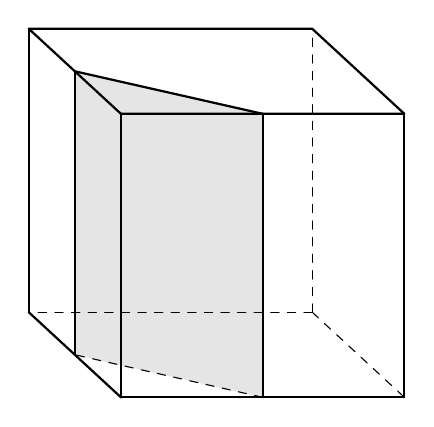
\begin{tikzpicture}[
  scale=0.9,
  line cap=round,
  line join=round
]
  % Вершины куба
  \coordinate (A)  at (0,0);
  \coordinate (B)  at (4,0);
  \coordinate (D)  at (-1.3,1.2);
  \coordinate (C)  at (2.7,1.2);

  \coordinate (A1) at (0,4);
  \coordinate (B1) at (4,4);
  \coordinate (D1) at (-1.3,5.2);
  \coordinate (C1) at (2.7,5.2);

  % Середины
  \coordinate (M)  at (2,0);
  \coordinate (N)  at (-0.65,0.6);
  \coordinate (M1) at (2,4);
  \coordinate (N1) at (-0.65,4.6);

  % Плоскость сечения
  \fill[black!10] (M)--(N)--(N1)--(M1)--cycle;

  % Куб
  \draw[thick] (A)--(B);
  \draw[dashed] (C)--(D);
  \draw[thick] (A)--(D);
  \draw[dashed] (C)--(B);
  \draw[thick] (A1)--(B1)--(C1)--(D1)--cycle;
  \draw[thick] (A)--(A1);
  \draw[thick] (B)--(B1);
  \draw[dashed] (C)--(C1);
  \draw[thick] (D)--(D1);

  % Отсекаемая треугольная призма

  \draw[thick] (A)--(A1);
  \draw[thick] (M)--(M1);
  \draw[thick] (N)--(N1);

  % След плоскости
  \draw[dashed] (M)--(N);
  \draw[thick] (M1)--(N1);
\end{tikzpicture}
\end{center}
\section*{Вариант 26}

\textbf{5.} Объём треугольной призмы, отсекаемой от куба плоскостью,
проходящей через середины двух рёбер, выходящих из одной вершины,
и параллельной третьему ребру, выходящему из этой же вершины,
равен \(11\). Найдите объём куба.

\begin{center}
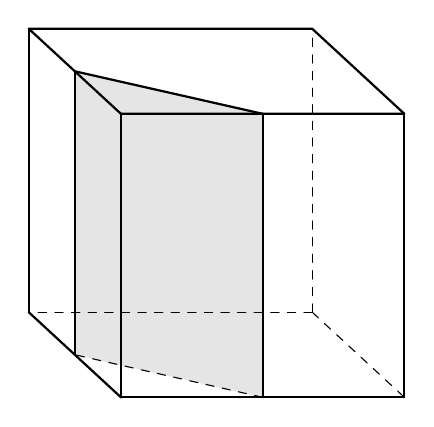
\begin{tikzpicture}[
  scale=0.9,
  line cap=round,
  line join=round
]
  % Вершины куба
  \coordinate (A)  at (0,0);
  \coordinate (B)  at (4,0);
  \coordinate (D)  at (-1.3,1.2);
  \coordinate (C)  at (2.7,1.2);

  \coordinate (A1) at (0,4);
  \coordinate (B1) at (4,4);
  \coordinate (D1) at (-1.3,5.2);
  \coordinate (C1) at (2.7,5.2);

  % Середины
  \coordinate (M)  at (2,0);
  \coordinate (N)  at (-0.65,0.6);
  \coordinate (M1) at (2,4);
  \coordinate (N1) at (-0.65,4.6);

  % Плоскость сечения
  \fill[black!10] (M)--(N)--(N1)--(M1)--cycle;

  % Куб
  \draw[thick] (A)--(B);
  \draw[dashed] (C)--(D);
  \draw[thick] (A)--(D);
  \draw[dashed] (C)--(B);
  \draw[thick] (A1)--(B1)--(C1)--(D1)--cycle;
  \draw[thick] (A)--(A1);
  \draw[thick] (B)--(B1);
  \draw[dashed] (C)--(C1);
  \draw[thick] (D)--(D1);

  % Отсекаемая треугольная призма

  \draw[thick] (A)--(A1);
  \draw[thick] (M)--(M1);
  \draw[thick] (N)--(N1);

  % След плоскости
  \draw[dashed] (M)--(N);
  \draw[thick] (M1)--(N1);
\end{tikzpicture}
\end{center}
\section*{Вариант 27}

\textbf{5.} От треугольной пирамиды, объём которой равен \(42\), отсечена
треугольная пирамида плоскостью, проходящей через вершину пирамиды
и среднюю линию основания. Найдите объём отсечённой треугольной пирамиды.

\begin{center}
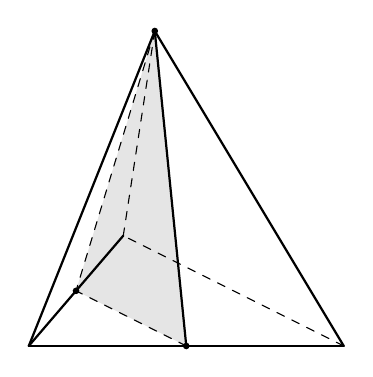
\begin{tikzpicture}[
  scale=1,
  line cap=round,
  line join=round
]
  % Основание
  \coordinate (A) at (0,0);
  \coordinate (B) at (4,0);
  \coordinate (C) at (1.2,1.4);

  % Вершина
  \coordinate (S) at (1.6,4);

  % Средняя линия основания
  \coordinate (M) at (2,0);      % середина AB
  \coordinate (N) at (0.6,0.7);  % середина AC

  % Полупрозрачная секущая плоскость
  \fill[black!10] (S)--(M)--(N)--cycle;

  % Основание пирамиды
  \draw[thick] (A)--(B);
  \draw[thick] (A)--(C);
  \draw[dashed] (B)--(C);

  % Боковые рёбра
  \draw[thick] (S)--(A);
  \draw[thick] (S)--(B);
  \draw[dashed] (S)--(C);

  % Грани отсечённой пирамиды / след плоскости
  \draw[thick] (S)--(M);
  \draw[dashed] (S)--(N);
  \draw[dashed] (M)--(N);

  \fill (S) circle (1.2pt);
  \fill (M) circle (1.2pt);
  \fill (N) circle (1.2pt);
\end{tikzpicture}
\end{center}
\section*{Вариант 28}

\textbf{5.} Найдите объём правильной треугольной пирамиды, стороны основания
которой равны \(12\), а высота равна \(6\sqrt{3}\).

\begin{center}
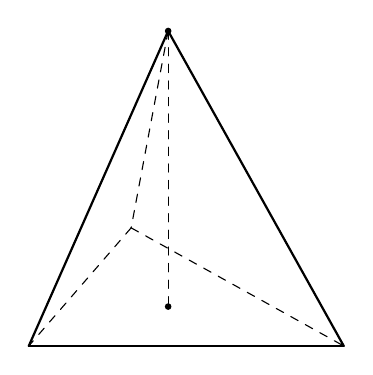
\begin{tikzpicture}[
  scale=1,
  line cap=round,
  line join=round
]
  % Основание
  \coordinate (A) at (0,0);
  \coordinate (B) at (4,0);
  \coordinate (C) at (1.3,1.5);

  % Центр основания
  \coordinate (O) at (1.77,0.5);

  % Вершина
  \coordinate (S) at (1.77,4);

  % Основание
  \draw[thick] (A)--(B);
  \draw[dashed] (C)--(B);
  \draw[dashed] (C)--(A);

  % Боковые рёбра
  \draw[thick] (S)--(A);
  \draw[thick] (S)--(B);
  \draw[dashed] (S)--(C);

  % Высота
  \draw[dashed] (S)--(O);

  \fill (S) circle (1.2pt);
  \fill (O) circle (1.2pt);
\end{tikzpicture}
\end{center}

\section*{Вариант 29}

\textbf{5.} Шар, объём которого равен \(64\), вписан в цилиндр.
Найдите объём цилиндра.

\begin{center}
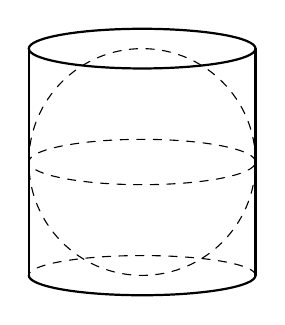
\begin{tikzpicture}[
  scale=0.9,
  line cap=round,
  line join=round
]
  \def\R{1.6}
  \def\H{3.2}
  \def\e{0.28}

  \coordinate (O) at (0,1.6);

  % Шар
  \draw[dashed] (O) circle (\R);
  \draw[dashed]
    (O) ellipse[x radius=\R,y radius=0.32];

  % Верхнее основание цилиндра
  \draw[thick]
    (0,\H) ellipse[x radius=\R,y radius=\e];

  % Образующие цилиндра
  \draw[thick] (-\R,0)--(-\R,\H);
  \draw[thick] ( \R,0)--( \R,\H);

  % Нижнее основание цилиндра
  \draw[thick]
    (-\R,0)
    arc[
      start angle=180,
      end angle=360,
      x radius=\R,
      y radius=\e
    ];

  \draw[dashed]
    (\R,0)
    arc[
      start angle=0,
      end angle=180,
      x radius=\R,
      y radius=\e
    ];
\end{tikzpicture}
\end{center}
\section*{Вариант 30}

\textbf{5.} Шар вписан в цилиндр. Площадь поверхности шара равна \(74\).
Найдите площадь полной поверхности цилиндра.

\begin{center}
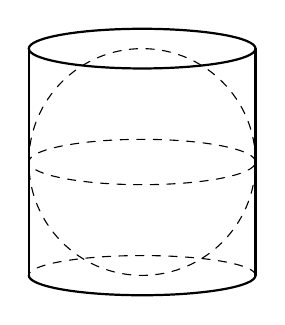
\begin{tikzpicture}[
  scale=0.9,
  line cap=round,
  line join=round
]
  \def\R{1.6}
  \def\H{3.2}
  \def\e{0.28}

  \coordinate (O) at (0,1.6);

  % Шар
  \draw[dashed] (O) circle (\R);
  \draw[dashed]
    (O) ellipse[x radius=\R,y radius=0.32];

  % Верхнее основание цилиндра
  \draw[thick]
    (0,\H) ellipse[x radius=\R,y radius=\e];

  % Образующие цилиндра
  \draw[thick] (-\R,0)--(-\R,\H);
  \draw[thick] ( \R,0)--( \R,\H);

  % Нижнее основание цилиндра
  \draw[thick]
    (-\R,0)
    arc[
      start angle=180,
      end angle=360,
      x radius=\R,
      y radius=\e
    ];

  \draw[dashed]
    (\R,0)
    arc[
      start angle=0,
      end angle=180,
      x radius=\R,
      y radius=\e
    ];
\end{tikzpicture}
\end{center}
\section*{Вариант 31}

\textbf{5.} В правильной четырёхугольной пирамиде \(SABCD\)
точка \(O\) --- центр основания, \(S\) --- вершина,
\(SO=9\), \(SC=15\). Найдите длину отрезка \(BD\).

\begin{center}
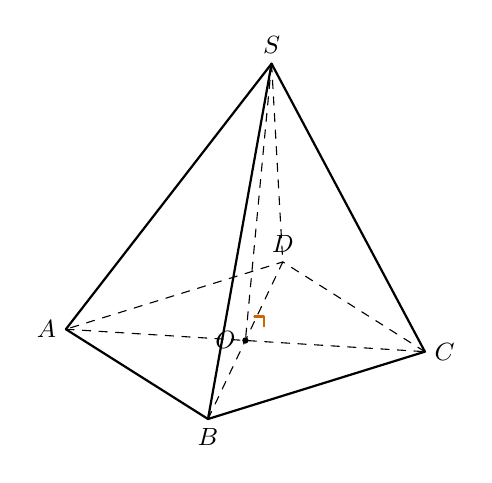
\begin{tikzpicture}[
  scale=0.95,
  line cap=round,
  line join=round,
  every node/.style={font=\small}
]
  % Основание (развёрнуто так, чтобы внутренние линии были лучше видны)
  \coordinate (A) at (-2.6,-0.35);
  \coordinate (B) at (-0.7,-1.55);
  \coordinate (C) at (2.2,-0.65);
  \coordinate (D) at (0.3,0.55);

  % Центр основания
  \coordinate (O) at (-0.2,-0.5);

  % Вершина
  \coordinate (S) at (0.15,3.2);

  % Видимые стороны основания
  \draw[thick] (A)--(B)--(C);

  % Скрытые стороны основания
  \draw[dashed] (C)--(D)--(A);

  % Боковые рёбра
  \draw[thick] (S)--(A);
  \draw[thick] (S)--(B);
  \draw[thick] (S)--(C);
  \draw[dashed] (S)--(D);

  % Диагонали основания
  \draw[dashed] (A)--(C);
  \draw[dashed] (B)--(D);

  % Высота
  \draw[dashed] (S)--(O);

  % Точки
  \fill (O) circle (1.2pt);

  % Значок прямого угла у O
  \draw[orange!80!black, thick]
    (-0.08,-0.18) -- (0.05,-0.18) -- (0.05,-0.31);

  % Подписи
  \node[left]  at (A) {$A$};
  \node[below] at (B) {$B$};
  \node[right] at (C) {$C$};
  \node[above] at (D) {$D$};
  \node[left]  at (O) {$O$};
  \node[above] at (S) {$S$};
\end{tikzpicture}
\end{center}
\section*{Вариант 32}

\textbf{5.} Шар вписан в цилиндр. Площадь поверхности шара равна \(26\).
Найдите площадь полной поверхности цилиндра.

\begin{center}
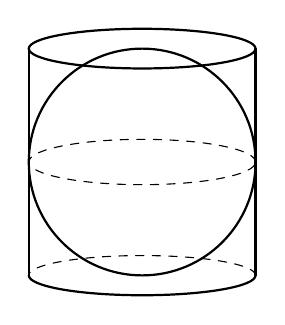
\begin{tikzpicture}[
  scale=0.9,
  line cap=round,
  line join=round
]
  \def\R{1.6}
  \def\H{3.2}
  \def\e{0.28}

  \coordinate (O) at (0,1.6);

  % Шар
  \draw[thick] (O) circle (\R);
  \draw[dashed]
    (O) ellipse[x radius=\R,y radius=0.32];

  % Верхнее основание цилиндра
  \draw[thick]
    (0,\H) ellipse[x radius=\R,y radius=\e];

  % Образующие цилиндра
  \draw[thick] (-\R,0)--(-\R,\H);
  \draw[thick] ( \R,0)--( \R,\H);

  % Нижнее основание цилиндра
  \draw[thick]
    (-\R,0)
    arc[
      start angle=180,
      end angle=360,
      x radius=\R,
      y radius=\e
    ];

  \draw[dashed]
    (\R,0)
    arc[
      start angle=0,
      end angle=180,
      x radius=\R,
      y radius=\e
    ];
\end{tikzpicture}
\end{center}
\section*{Вариант 33}

\textbf{5.} Найдите объём многогранника, вершинами которого являются
вершины \(A\), \(B\), \(C\), \(D\), \(B_1\) прямоугольного параллелепипеда
\(ABCDA_1B_1C_1D_1\), у которого
\(AB=9\), \(BC=3\), \(BB_1=8\).

\begin{center}
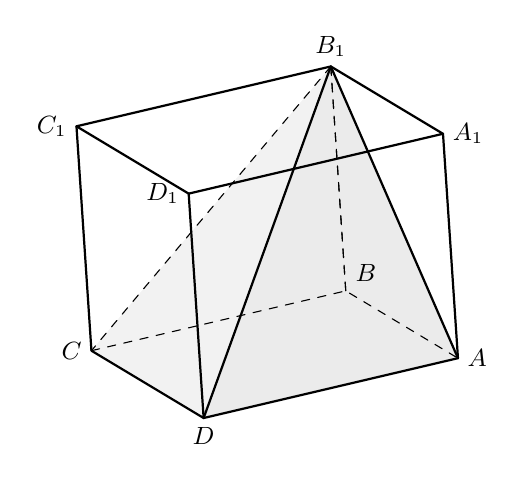
\begin{tikzpicture}[
  scale=0.95,
  line cap=round,
  line join=round,
  every node/.style={font=\small}
]
  % Нижнее основание параллелепипеда
  % Фигура специально развёрнута:
  % вершины B и D не лежат на одной вертикали
  \coordinate (A) at ( 2.7, 0.1);
  \coordinate (B) at ( 1.2, 1.0);
  \coordinate (C) at (-2.2, 0.2);
  \coordinate (D) at (-0.7,-0.7);

  % Верхнее основание
  \coordinate (A1) at ( 2.5,3.1);
  \coordinate (B1) at ( 1.0,4.0);
  \coordinate (C1) at (-2.4,3.2);
  \coordinate (D1) at (-0.9,2.3);

  % Полупрозрачные грани искомого многогранника ABCDB_1
  \fill[black!5]
    (B1)--(C)--(D)--cycle;

  \fill[black!8]
    (B1)--(D)--(A)--cycle;

  % Нижнее основание:
  % передние рёбра
  \draw[thick] (C)--(D)--(A);

  % задние рёбра
  \draw[dashed] (C)--(B)--(A);

  % Верхнее основание параллелепипеда
  \draw[thick]
    (C1)--(B1)--(A1)--(D1)--cycle;

  % Боковые рёбра параллелепипеда
  \draw[thick]  (C)--(C1);
  \draw[thick]  (D)--(D1);
  \draw[thick]  (A)--(A1);
  \draw[dashed] (B)--(B1);

  % Рёбра искомого многогранника
  \draw[dashed] (B1)--(C);
  \draw[thick] (B1)--(D);
  \draw[thick] (B1)--(A);

  % Скрытое ребро B_1B
  \draw[dashed] (B1)--(B);

  % Подписи нижнего основания
  \node[right]       at (A) {$A$};
  \node[above right] at (B) {$B$};
  \node[left]        at (C) {$C$};
  \node[below]       at (D) {$D$};

  % Подписи верхнего основания
  \node[right] at (A1) {$A_1$};
  \node[above] at (B1) {$B_1$};
  \node[left]  at (C1) {$C_1$};
  \node[left]  at (D1) {$D_1$};
\end{tikzpicture}
\end{center}
\section*{Вариант 35}

\textbf{5.} Площадь боковой поверхности конуса равна \(30\).
Параллельно основанию конуса проведено сечение,
делящее высоту в отношении \(2:3\), считая от вершины конуса.
Найдите площадь боковой поверхности отсечённого конуса.

\begin{center}
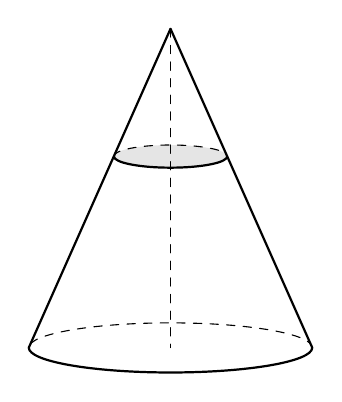
\begin{tikzpicture}[
  scale=0.9,
  line cap=round,
  line join=round
]
  \def\R{2}
  \def\e{0.35}

  \coordinate (S) at (0,4.5);
  \coordinate (L) at (-\R,0);
  \coordinate (R) at ( \R,0);
  \coordinate (O) at (0,0);

  % Центр секущей плоскости
  \coordinate (Q) at (0,2.7);

  % Полупрозрачное сечение
  \fill[black!10]
    (Q) ellipse[x radius=0.8,y radius=0.16];

  % Образующие конуса
  \draw[thick] (S)--(L);
  \draw[thick] (S)--(R);

  % Основание конуса
  \draw[thick]
    (L)
    arc[
      start angle=180,
      end angle=360,
      x radius=\R,
      y radius=\e
    ];

  \draw[dashed]
    (R)
    arc[
      start angle=0,
      end angle=180,
      x radius=\R,
      y radius=\e
    ];

  % Видимая часть линии сечения
  \draw[thick]
    (0.8,2.7)
    arc[
      start angle=0,
      end angle=-180,
      x radius=0.8,
      y radius=0.16
    ];

  % Скрытая часть линии сечения
  \draw[dashed]
    (-0.8,2.7)
    arc[
      start angle=180,
      end angle=0,
      x radius=0.8,
      y radius=0.16
    ];

  % Высота конуса
  \draw[dashed] (S)--(O);
\end{tikzpicture}
\end{center}
\section*{Вариант 36}

\textbf{5.} В основании прямой призмы лежит прямоугольный треугольник
с катетами \(5\) и \(6\). Боковые рёбра призмы равны
\(\frac{4}{\pi}\).
Найдите объём цилиндра, описанного около этой призмы.

\begin{center}
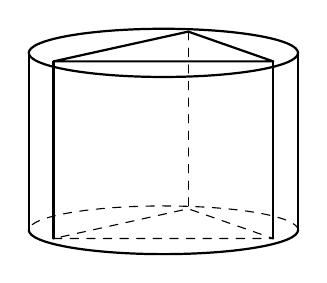
\begin{tikzpicture}[
  scale=0.9,
  line cap=round,
  line join=round
]
  \def\R{1.9}
  \def\H{2.5}
  \def\e{0.34}

  % Вершины верхнего основания призмы
  \coordinate (T1) at (-1.55,2.38);
  \coordinate (T2) at ( 1.55,2.38);
  \coordinate (T3) at ( 0.35,2.80);

  % Вершины нижнего основания призмы
  \coordinate (B1) at (-1.55,-0.12);
  \coordinate (B2) at ( 1.55,-0.12);
  \coordinate (B3) at ( 0.35, 0.30);

  % Верхнее основание цилиндра
  \draw[thick]
    (0,\H) ellipse[x radius=\R,y radius=\e];

  % Образующие цилиндра
  \draw[thick] (-\R,0)--(-\R,\H);
  \draw[thick] ( \R,0)--( \R,\H);

  % Нижнее основание цилиндра
  \draw[thick]
    (-\R,0)
    arc[
      start angle=180,
      end angle=360,
      x radius=\R,
      y radius=\e
    ];

  \draw[dashed]
    (\R,0)
    arc[
      start angle=0,
      end angle=180,
      x radius=\R,
      y radius=\e
    ];

  % Верхнее основание призмы
  \draw[thick]
    (T1)--(T2)--(T3)--cycle;

  % Нижнее основание призмы
  \draw[dashed]
    (B1)--(B2)--(B3)--cycle;

  % Боковые рёбра призмы
  \draw[thick]  (T1)--(B1);
  \draw[thick]  (T2)--(B2);
  \draw[dashed] (T3)--(B3);
\end{tikzpicture}
\end{center}


